
\documentclass{beamer}

%% TODO: Uncomment the next three lines to add notes to presentation slides
%\usepackage{pgfpages}
%\setbeameroption{show notes on second screen}
%\setbeamertemplate{note page}{\insertnote}

\usepackage[utf8]{inputenc}

\usepackage{graphicx}

\usepackage{tabularx}

\graphicspath{{images/}}

\usepackage{amsmath}
\usepackage{amssymb}
\usepackage{tikz}  
\usetikzlibrary{shapes, arrows.meta, positioning}  

\usepackage{pifont}

%% TODO: Use \cmark for tick and \xmark for x
\newcommand{\cmark}{\ding{51}}%
\newcommand{\xmark}{\ding{55}}%

\usepackage{algorithm}
\usepackage{algpseudocode}

\usepackage{lmodern}
\usepackage[T1]{fontenc}
\usepackage{booktabs}
\usepackage{amsmath}


%% TODO: Comment the next three lines to remove the bibliography
\usepackage[backend=biber,style=numeric, citestyle=ieee]{biblatex}
\addbibresource{bibliography.bib}
\AtBeginBibliography{\small}

\usepackage{appendixnumberbeamer}
\pdfstringdefDisableCommands{%
\def\translate#1{#1}%
}

\usepackage[most]{tcolorbox}

\newtcolorbox{simplebox}[1]{  
  title=#1,               % Title from argument  
  colback=blue!10,        % Light blue background  
  colframe=blue!70!black, % Dark blue frame  
  fonttitle=\bfseries,    % Bold title  
  boxrule=0pt,            % No frame around the text area  
  toprule=2mm,            % Thick rule at the top (blue band)  
  enhanced,               % Required for shadow  
  drop shadow             % Simple shadow with default settings  
}  

\newtcolorbox{plusbox}[1]{  
  title=#1,               % Title from argument  
  colback=green!10,        % Light blue background  
  colframe=green!70!black, % Dark blue frame  
  fonttitle=\bfseries,    % Bold title  
  boxrule=0pt,            % No frame around the text area  
  toprule=2mm,            % Thick rule at the top (blue band)  
  enhanced,               % Required for shadow  
  drop shadow             % Simple shadow with default settings  
}  

\newtcolorbox{minusbox}[1]{  
  title=#1,               % Title from argument  
  colback=green!10,        % Light blue background  
  colframe=green!70!black, % Dark blue frame  
  fonttitle=\bfseries,    % Bold title  
  boxrule=0pt,            % No frame around the text area  
  toprule=2mm,            % Thick rule at the top (blue band)  
  enhanced,               % Required for shadow  
  drop shadow             % Simple shadow with default settings  
}  

\beamertemplatenavigationsymbolsempty

\usetheme{Berlin}
\useinnertheme{circles}

\AtBeginSection[]
{
 \begin{frame}
 \frametitle{Table of Contents}
 \tableofcontents[currentsection]
 \end{frame}
}

%% TODO: Add information to the title page
\title{\textbf{An Estimated Dynamic Stochastic General Equilibrium Model of the Euro Area}}  
  
\subtitle{Frank Smets \& Raf Wouters\\[1ex]  
\rule{8cm}{0.5pt}}  
  
\author{Lauri HANNIKAINEN \\ Romain FERNEX}  
  
\institute[SciencesPo Paris]{SciencesPo Paris}  
  
\date[Thesis Defense]{Master in Economics}  
   

%% Page number
\expandafter\def\expandafter\insertshorttitle\expandafter{%
 \insertshorttitle\hfill%
 \insertframenumber\,/\,\inserttotalframenumber}

\makeatletter  
\setbeamertemplate{title page}{  
  \vbox{}  
  \vfill  
  \begingroup  
    % Title box with increased vertical padding and middle alignment  
    \begin{beamercolorbox}[wd=\paperwidth,sep=15pt,leftskip=1cm,rightskip=1cm,center,middle]{title}  
      \usebeamerfont{title}\inserttitle\par%  
      \ifx\insertsubtitle\@empty%  
      \else%  
        \vskip0.5em%  
        {\usebeamerfont{subtitle}\usebeamercolor[fg]{subtitle}\insertsubtitle\par}%  
      \fi%  
    \end{beamercolorbox}%  
    \vskip1em%  
    \begin{beamercolorbox}[sep=8pt,center]{author}  
      \usebeamerfont{author}\insertauthor  
    \end{beamercolorbox}  
    \begin{beamercolorbox}[sep=8pt,center]{institute}  
      \usebeamerfont{institute}\insertinstitute  
    \end{beamercolorbox}  
    \begin{beamercolorbox}[sep=8pt,center]{date}  
      \usebeamerfont{date}\insertdate  
    \end{beamercolorbox}  
  \endgroup  
  \vfill  
}  
\makeatother  

\begin{document}

%% Title frame
\begin{frame}
	\titlepage
\end{frame}

%% ToC frame
\begin{frame}{Table of Contents}
	\tableofcontents
	%% TODO: You can add the note here
	\note{}
\end{frame}

\section{Introduction} 

\begin{frame}{Motivation : Why this study ?}
    \begin{center}  
        \Large\textbf{Key Objectives}  
    \end{center}  
    \vspace{0.5em}
	\begin{itemize} 	
		\item Establish and estimate a \textbf{new DSGE} (Dynamic stochastic general equilibrium) model for the Euro Area with both price and \textbf{wage stickiness} as well as additional features such as partial \textbf{indexation} and external \textbf{habit formation}. 
		\item \textbf{Compare} this model to benchmarks (VAR), \textbf{estimate} impulse responses for a large panel of \textbf{structural shocks} ($>11$ shocks) and investigate the main contributors of \textbf{variance} in output and inflation through a variance and a historical \textbf{decomposition}.
	\end{itemize}
\end{frame}

\begin{frame}[label=objectives]{Methods: How do they obtain their results?}    
  \setlength{\parskip}{0pt}    
  \setlength{\topsep}{0pt}    
    \vspace{-0.3cm}
  \begin{simplebox}{A Bayesian Model}    
    \footnotesize  
    \textbf{Bayesian approach} to find the posterior distribution of endogenous variables using \textbf{empirical data from the Euro Area}.  
  \end{simplebox}  
  
  \begin{simplebox}{Estimation/Calibration Method}    
    \footnotesize  
    The model is estimated using the Bayesian estimation/calibration method instead of more traditional methods like GMM for better \textbf{model fit}.  
  \end{simplebox}  
  
  \begin{simplebox}{Decomposition Method}    
    \footnotesize  
    \textbf{Variance :} Studies the contribution of structural shocks to the variance in the \textbf{predicted endogenous variables} by looking at \textbf{forecast errors.} 
  \end{simplebox}    
\end{frame}    

\begin{frame}{Results: What did the Authors Find?}   
    \begin{itemize}    
        \item \textbf{Model Comparison:}    
        \begin{itemize}    
            \item The model performs \textbf{at least as well as most existing models (VARs and BVARs)}.  
        \end{itemize}    
            
        \vspace{0.5em}    
            
        \item \textbf{Impulse Responses:}    
        \begin{itemize}    
            \item Adding the 11 proposed structural shocks enables the model to \textbf{match data} much \textbf{more effectively} than models incorporating a limited variety of shocks.  
        \end{itemize}    
            
        \vspace{0.5em}    
            
        \item \textbf{Variance Decomposition:}    
        \begin{itemize}    
            \item \textbf{Output} fluctuations are primarily explained by: \textbf{labor \& monetary} shocks + fiscal shocks (in the \textbf{short run}) and \textbf{not by productivity shocks} as proposed in earlier studies.  
            \item \textbf{Inflation} variations are driven by: \textbf{price markup} shocks + monetary policy (in the \textbf{medium/long run}).  
        \end{itemize}    
    \end{itemize}    
\end{frame}  

\section{Model}


\begin{frame}{New Model Features}
    \begin{center}  
        \Large\textbf{New Model Features}  
    \end{center}  
    \vspace{0.5em}
    \renewcommand{\arraystretch}{1.2}
    \centering
    \begin{tabularx}{\linewidth}{p{4.3cm} X}
    \toprule
    \textbf{Model Feature} & \textbf{Implementation} \\
    \midrule
    \textbf{External Habit in Consumption} 
    & Utility depends on $C_t - h\,C_{t-1}$ \\[1ex]
    \textbf{Investment Adjustment Cost} 
    & Adjustment cost $\propto \left(\frac{I_t}{I_{t-1}}-1\right)^2$ \\[1ex]
    \textbf{Variable Capacity      Utilization} 
    & Firms choose utilization $u_t$; $\hat{u}_t = \psi\,\hat{r}^K_t$, with capital services $u_tK_{t-1}$. \\[1ex]
    \textbf{Calvo Wage Stickiness} 
    & A fraction $\xi_w$ of households do not adjust wages.\\
    \bottomrule
    \end{tabularx}
\end{frame}


\begin{frame}{Structural Shock Processes}
 
    \vspace{0.1em}
    \renewcommand{\arraystretch}{0.8}
    \centering
    \begin{tabularx}{\linewidth}{p{3.5cm} X}
    \toprule
    \textbf{Shock Name} & \textbf{Explanation} \\
    \midrule
    TFP Shock & $\epsilon^a_t$ (AR(1), $\rho_a$) in production function \\[1ex]
    Preference Shock & $\epsilon^b_t$ (AR(1), $\rho_b$) in consumption Euler \\[1ex]
    Inv. Cost Shock & $\epsilon^I_t$ (AR(1), $\rho_I$) in investment equation \\[1ex]
    Labor Supply Shock & $\epsilon^L_t$ (AR(1), $\rho_L$) in wage eq. \\[1ex]
    Gov. Spending Shock & $\epsilon^G_t$ (AR(1), $\rho_G$) in resource constraint \\[1ex]
    Price Markup Shock & $\eta^p_t$ (i.i.d.) in inflation equation \\[1ex]
    Wage Markup Shock & $\eta^w_t$ (i.i.d.) in wage equation \\[1ex]
    Eq. Premium Shock & $\nu^Q_t$ (i.i.d.) in $Q$-equation \\[1ex]
    Mon. Policy Shock & $\eta^R_t$ (i.i.d.) in interest rule \\[1ex]
    Infl. Target Shock & $\pi^*_t$ (AR(1)) in interest rule \\
    \bottomrule
    \end{tabularx}
    
    \vspace{1em}
\end{frame}

\begin{frame}{Real wage equation}

\begin{itemize}    
        \item We assume that when a household cannot adjust their wage, they set their wage according to \[
W_t^{\tau} = \left(\frac{P_{t-1}}{P_{t-2}}\right)^{\gamma_w} \, W_{t-1}^{\tau}
\]  
     
            \item This yields the following  \textbf{real wage equation}  
\end{itemize}   


\begin{aligned}
\hat{w}_t 
&= \frac{\beta}{1 + \beta}\,E_t\bigl[\hat{w}_{t+1}\bigr]
   \;+\;\frac{1}{1 + \beta}\,\hat{w}_{t-1}
   \;+\;\frac{1}{1 + \beta}\,E_t\bigl[\hat{\pi}_{t+1}\bigr]
   \;-\;\frac{1 + \beta\,\gamma_w}{1 + \beta}\,\hat{\pi}_t \\[6pt]
&\quad +\;\frac{\gamma_w}{1 + \beta}\,\hat{\pi}_{t-1}
   \;+\;\frac{\bigl(1 - \beta\,\xi_w\bigr)\,\bigl(1 - \xi_w\bigr)}{\bigl(1 + \beta\bigr)\,\xi_w}
       \,\frac{\bigl(1 + \lambda_w\bigr)\,\sigma_L}{\bigl(1 + \lambda_w\bigr)\,\lambda_w} \\[6pt]
&\quad \times \Bigl[
     \hat{w}_t 
   \;-\;\sigma_L\,\hat{L}_t 
   \;-\;\frac{\sigma_c}{1 - h}\,\bigl(\hat{C}_t - h\,\hat{C}_{t-1}\bigr)
   \;-\;\epsilon^L_t 
   \;-\;\eta^w_t
\Bigr]
\end{aligned}

\end{frame}


%%%%%%%%%%%%%%%%

\begin{frame}{NKPC}

\begin{itemize}    
    \item Similarly, when a firm cannot adjust their price, they set the price to  \[
P_t^{\tau} = \left(\frac{P_{t-1}}{P_{t-2}}\right)^{\gamma_p} \, P_{t-1}^{\tau}
\]

    \vspace{0.5em}  
 
    \item This yields the following \textbf{New Keynesian Phillips Curve}
    \vspace{0.5em}  
 


\end{itemize}  
\begin{aligned}
\hat{\pi}_t 
&= \frac{\beta}{1 + \beta \gamma_p}\,E_t[\hat{\pi}_{t+1}]
  \;+\;\frac{\gamma_p}{1 + \beta \gamma_p}\,\hat{\pi}_{t-1} \\[6pt]
&\quad+\;\frac{1}{1 + \beta \gamma_p}\,\frac{(1 - \beta\,\xi_p)\,(1 - \xi_p)}{\xi_p}
   \,\Bigl[\alpha\,\hat{r}_t^k \;+\;(1-\alpha)\,\hat{w}_t \;-\;\epsilon_t^a \;+\;\eta_t^p\Bigr]
\end{aligned}

\end{frame}

		 
\section{A Bayesian Approach} 
%% I'm adding a small note on frequentist and bayesian statistics

\begin{frame}{What is the Bayesian Approach ? (1/3)}

    \begin{center}  
        \Large\textbf{Bayesian vs Frequentist}  
    \end{center}  
    \vspace{0.5em}

\begin{itemize}
    \item \textbf{Frequentist approach:}
     Assume data-generating process, assume that data is a realization of an unobserved population, maximize likelihood function to get a point estimate, and estimate standard errors. \textbf{Cannot make probability statements.} 
\end{itemize}

\begin{itemize}
    \item \textbf{Bayesian approach:}
     Assume that parameter is a random variable with a given distribution (prior), assume a conditional distribution for the data given parameters (likelihood function), use Bayes rule to calculate posterior (note that this can now be done fully computationally, no further assumptions needed). \textbf{Can make probability statements.}
\end{itemize}

\end{frame}

\begin{frame}{What is the Bayesian Approach ? (2/3)}  
\vspace{-0.3cm}
\begin{simplebox}{Reasoning in Distributions}  
\small % Reduce overall font size  
\textbf{Prior Distribution - $P(\theta)$}  
\begin{itemize}\setlength{\itemsep}{0pt} % Remove space between items  
        \item \footnotesize The researcher chooses a distribution for the model parameters. The prior quantifies the uncertainty regarding the parameters before accounting for the model structure and data. 
\end{itemize}  
  
\textbf{Likelihood function - $P(Data|\theta)$}  
\begin{itemize}\setlength{\itemsep}{0pt}  
    \item \footnotesize Measures how likely the realization of data is given the parameters.
\end{itemize}  
  
\textbf{Posterior Distribution}  
\begin{itemize}\setlength{\itemsep}{0pt}  
    \item \footnotesize Updated probability distribution of the parameters
    $$\scriptsize P(\theta|Data) = \frac{P(Data|\theta)P(\theta)}{P(Data)} $$
\end{itemize}  
\end{simplebox}  
\end{frame}  

\begin{frame}{What is the Bayesian Approach ? (3/3)}
\textbf{Reading Results :}
\begin{columns}
		\column{0.5\textwidth}
		\begin{figure}
			\centering
			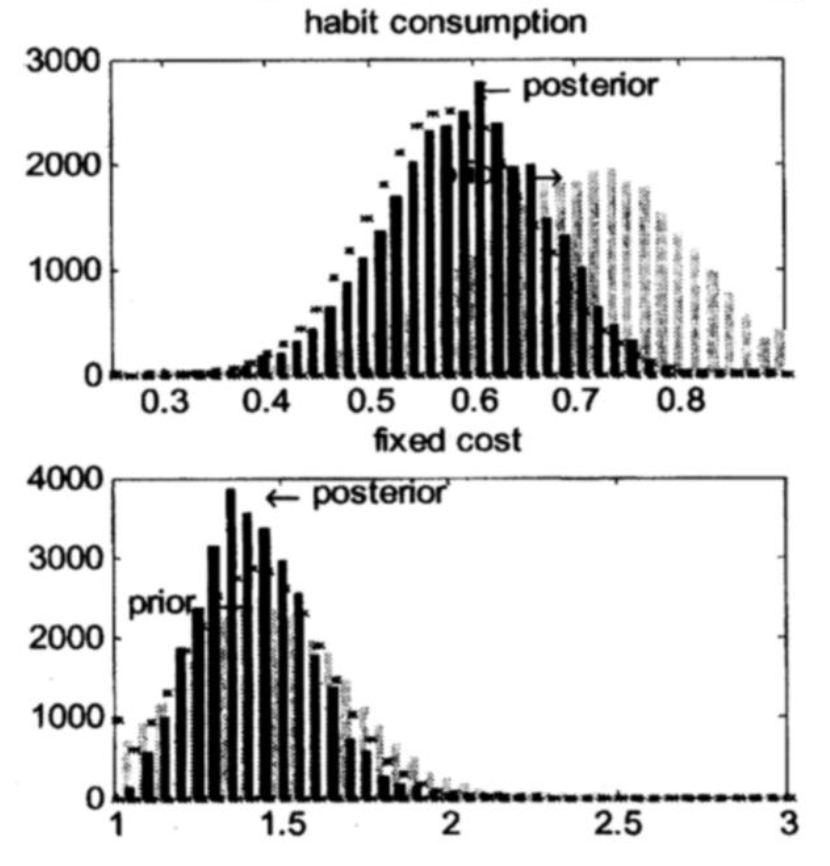
\includegraphics[width=.8\textwidth]{images/Estimation Parameters.png}
			\caption{Prior/Posterior distributions for some Parameters}
		\end{figure}	
		\column{0.5\textwidth}
		\begin{figure}
			\centering
			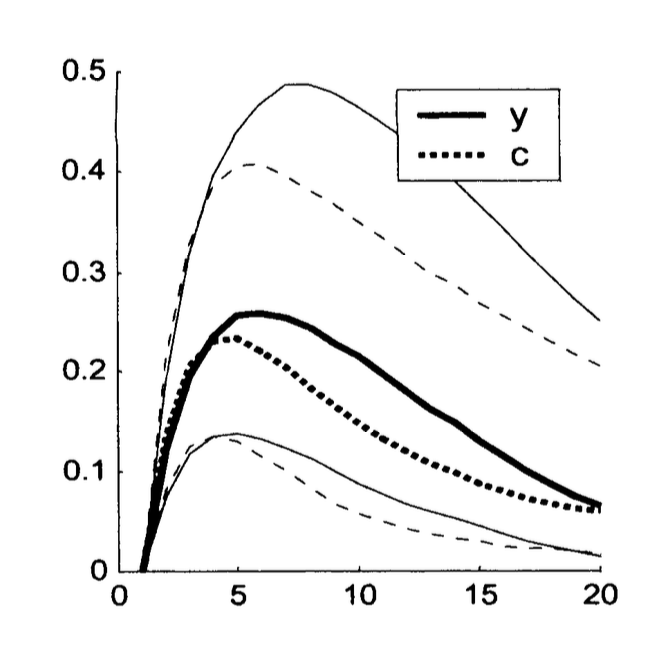
\includegraphics[width=.8\textwidth]{images/Estimation Variables.png}
			\caption{Model estimations of endogenous variables}
		\end{figure}
\end{columns}
\end{frame}

			
\section{Estimations} 
			
\begin{frame}{Calibrating the Model : Traditional Approach}		
\textbf{The Traditional Method :}
Use the General Method of Moment (GMM) to minimize a distance function between theoretical and empirical moments \\
\vspace{0.1cm}
\textbf{How does it work in practice ?}
\begin{enumerate}
    \item Theoretical impulse response functions are generated using the model 
    \item Empirical impulse response functions are estimated from the data
    \item Model parameters are adjusted to minimize the difference between both response functions
\end{enumerate}

\end{frame}

\begin{frame}{Calibrating the Model : The Author's Approach (1/2)}	
\begin{simplebox}{Bayesian Estimation}
Calibration is done through \textbf{likelihood maximization} using the likelihood function we introduced earlier. 
\end{simplebox}

\vspace{0.1cm}
\textbf{Key features}
\begin{itemize}
    \item Parameters are adjusted until the calculated likelihood function is as high as possible, meaning model prediction are close to real data
    \item No "one" best fit as range of likely parameter values are explored 
\end{itemize}
\end{frame}

\begin{frame}{Calibrating the Model: The Author's Approach (2/2)} 
\small{
\begin{enumerate}
    \item Simplify the model based on past data for the Euro Area
    \item Split the data between hidden  factors and real data
    \item Use the Kalman filter to match the observed data
    \item Adjust the model’s parameters by exploring a range of possibilities
\end{enumerate}}
{\small 
\begin{simplebox}{The Kalman Filter}  
Used to compare theoretical to empirical forecasts for hidden factors based on an observation equation.\\  {\normalsize\bfseries  
$$x_t=\hat{x}_t+K_t\Bigl(y_t-H F x_{t-1}\Bigr)$$  
}  
with $K_t$ the Kalman Gain (reliability), $H$ the observation matrix, and $F$ the state transition matrix.  
\end{simplebox}  
}  
\end{frame}  

\begin{frame}{Calibrating the model : Pros \& Cons of this approach}   
  \begin{columns}[T]    
    \column{0.48\textwidth}    
      \centering    
      \textcolor{green!60!black}{{\Large\bfseries Advantages}}\\[0.5em]    
      \begin{itemize}\setlength{\itemsep}{1em}    
          \item[\textcolor{green!60!black}{\large$\mathbf{+}$}] \normalsize \textbf{Incorporating uncertainty:} Can use full prior information coming from previous macro/microeconometric studies  
          \item[\textcolor{green!60!black}{\large$\mathbf{+}$}] \normalsize \textbf{Numerical Stability:} Using priors helps reduce instability linked to data scarcity     
      \end{itemize}    
          
    \column{0.48\textwidth}    
      \centering    
      \textcolor{red!60!black}{{\Large\bfseries Limitations}}\\[0.5em]    
      \begin{itemize}\setlength{\itemsep}{1em}    
          \item[\textcolor{red!60!black}{\large$\mathbf{-}$}] \normalsize \textbf{Prior sensitive:} It is not clear how priors affect the results    
          \item[\textcolor{red!60!black}{\large$\mathbf{-}$}] \normalsize \textbf{Practical use:} Reasoning in distribution sometimes leads to results that are hard to use for policy makers as they are not precise enough  
      \end{itemize}    
  \end{columns}    
\end{frame}

\begin{frame}{Estimation results : Impulse response functions}

\begin{columns}
\hspace{-0.5cm}
		\column{0.5\textwidth}
		\begin{figure}
			\centering
			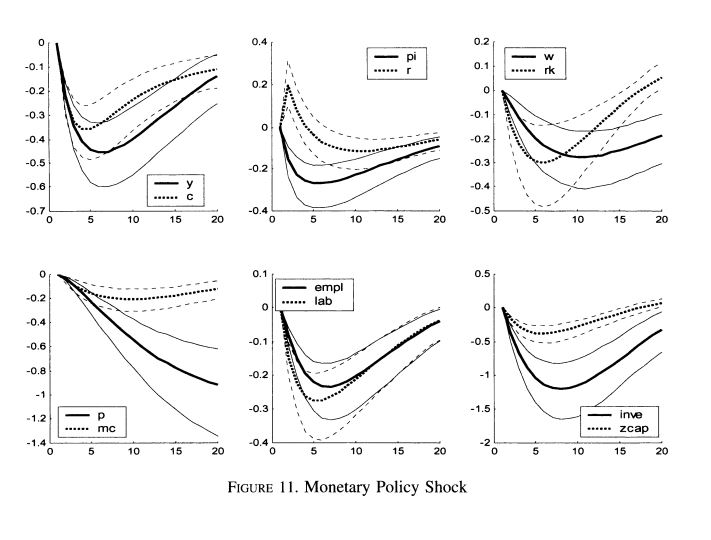
\includegraphics[width=1.1\textwidth]{images/IRF.JPG}
			\caption{\small Temporary Monetary Policy Shock}
		\end{figure}	
		\column{0.5\textwidth}
		\begin{figure}
			\centering
			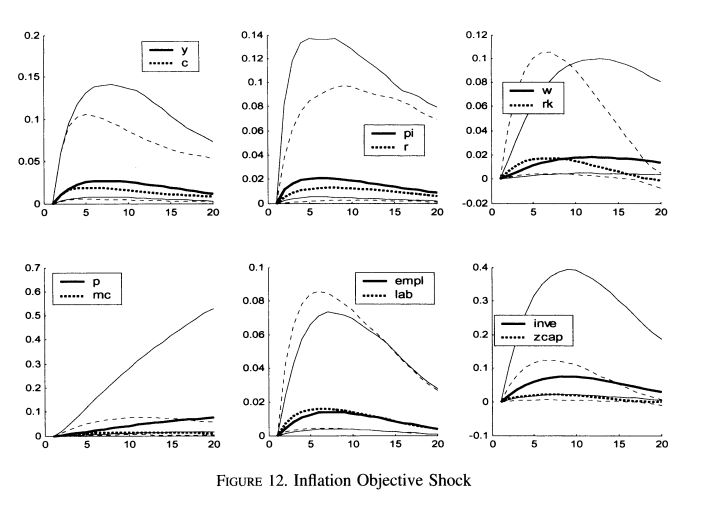
\includegraphics[width=1.1\textwidth]{images/irf inf obj.JPG}
			\caption{\small Persistent Monetary Policy (inflation objective) Shock}
		\end{figure}
\end{columns}

\end{frame} 

\section{Model Comparison} 

\begin{frame}{VAR(p)}
\begin{itemize}
    \item A bivariate (i.e., a two‐variable) first‐order VAR process (i.e., a VAR(1) process) is given as
    \[
    \begin{aligned}
    y_{1t} &= a_{11}\,y_{1,t-1} \;+\; a_{12}\,y_{2,t-1} \;+\; \epsilon_{1t},\\
    y_{2t} &= a_{21}\,y_{1,t-1} \;+\; a_{22}\,y_{2,t-1} \;+\; \epsilon_{2t},
    \end{aligned}
    \]
    where $\epsilon_{1t}$ and $\epsilon_{2t}$ are two error terms (independent of the history of $y_{1t}$ and $y_{2t}$) that may be correlated.
\end{itemize}

\begin{itemize}
    \item The idea of the VAR($p$) model is to regress each component of $\mathbf{y}_t$ on its own lags and on the lags of the other components.
    \item The model can describe lagged or dynamic dependencies among variables. For example, one may ask how $y_{2t}$ affects the future path of $y_{1t}$, and vice versa.
\end{itemize}
\end{frame}

\begin{frame}{Comparison Table}
\begin{figure}
    \centering
    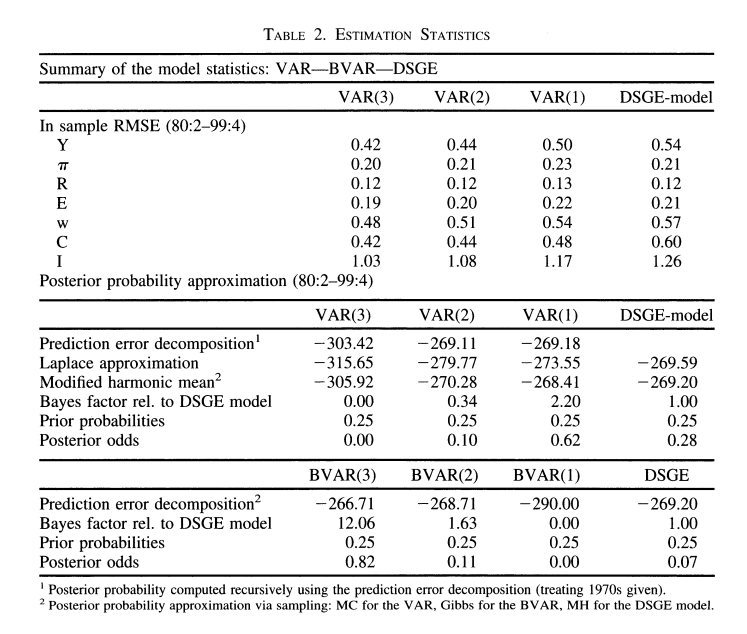
\includegraphics[width=1\linewidth]{images/comparison_table.png}
    \label{fig:enter-label}
\end{figure}
\end{frame}


\section{Variance Decomposition}
			
\begin{frame}{Variance Decomposition : Method}
\begin{itemize}
    \item \textbf{Goal :}  Quantify the \textbf{average expected contribution} of each structural shock to the forecast error variance\footnote{expected squared difference between the actual value and the predicted value of an endogenous variable ($E[(y_t-\hat{y}_t)^2]$)} of endogenous variables at \textbf{different time horizons}
    \item \textbf{Main attributes : } forward-looking, horizon-dependent
\end{itemize}
\vspace{0.5cm}
$$
    VD_{i,h} = \frac{\text{Variance due to shock i}}{\text{Total forecast error variance at horizon h}} \times 100\%
$$
\begin{itemize}
    \item \textbf{Simple interpretation :} the \textbf{larger} the \% of variance explained, the \textbf{bigger the impact} of a shock on the variable considered
\end{itemize}

\end{frame}
					
\begin{frame}{Variance Decomposition : Results}
    \begin{columns}  
        \column{0.01\textwidth} % Adjust this small value to shift left  
        \column{1.1\textwidth}  
        \begin{figure}  
            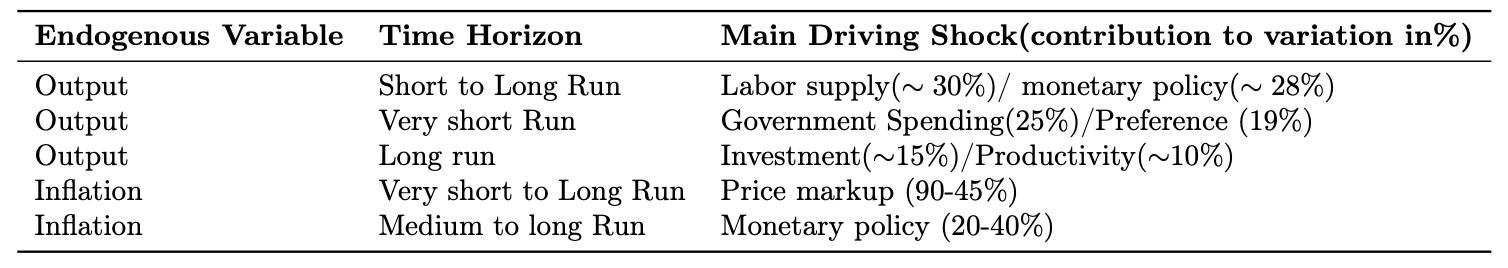
\includegraphics[width=\linewidth]{images/table_var_decomp.png}  
            \vspace{-0.6cm}  
            \small{\caption{Variance Decomposition Summary Table}}
            \label{fig:var decomp}  
        \end{figure}  
    \end{columns}  
\textbf{Main Observations}
\small{
    \begin{itemize}
        \item \textbf{Output :} Supply, productivity and Labor contribute to less than 40\% of the variance in output in the long-run compared to 45\% for labor alone with VARs (\cite{Shapiro:89}).
        \item \textbf{Inflation :} Monetary policy has a huge influence on the importance of the impact of other shocks on inflation. 
    \end{itemize}
}
\end{frame}

\begin{frame}{Historical Decomposition : Method}
\vspace{-0.3cm}
\begin{itemize}
    \item \textbf{Goal :} Rebuild the Shock paths that represent historical realizations
    \item \textbf{How does it Work ?} 
    \begin{enumerate}
        \item Start with the impulse response functions based on the model
        \item Infer the sequence of shocks that best explains movements in the observed data
    \end{enumerate}
    \item \textbf{Formula}\footnote{Source : course on Structural VAR by Aurélien Poissonnier(ENSAE)}
\end{itemize}
$$y_t = (\sum_{k=0}^{t-1}a_1^k)a_0 + a_t'y_0+\underbrace{\sum_{k=0}^{t-1}a_1^kS\epsilon_{t-k}}_{\text{Shock Contribution}}$$
\small{\hspace{0.6cm}With $S$ the weight matrix for the different shocks and $y_t=a_0 + a_1y_{t-1}+S\epsilon_t$}

\end{frame}
	
\begin{frame}{Historical Decomposition : Results}
\vspace{-0.3cm}
\begin{figure}
    \centering
    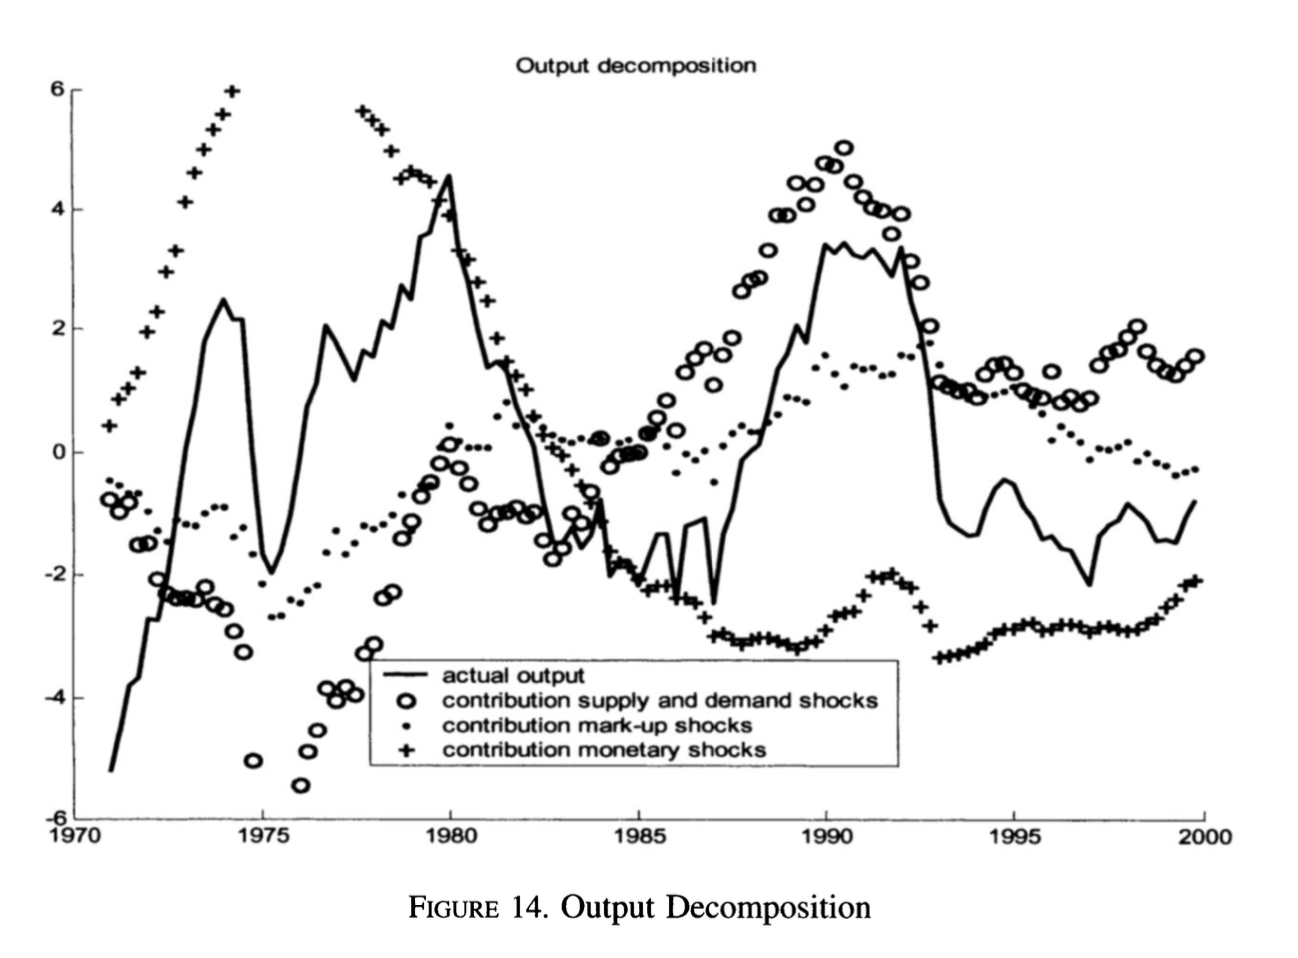
\includegraphics[width=0.9\linewidth]{images/hist_decomp_Y.png}
    \label{fig:enter-label}
\end{figure}

\end{frame}

\section{Discussion}

\begin{frame}{The Prediction Problem(1/2)}
\begin{simplebox}{Limitation n°1 : Wide prediction bands}
\textbf{Reasons:}
\begin{enumerate}
    \item\textbf{Short time frame:} The model is estimated on data over 1980:2-1999:4
    \item\textbf{High number of estimated parameters and shocks considered} 

\end{enumerate}
\end{simplebox}
\end{frame}

\begin{frame}{The Prediction Problem(2/2)}

\vspace{-0.1cm}  
\begin{figure}  
    \centering  
    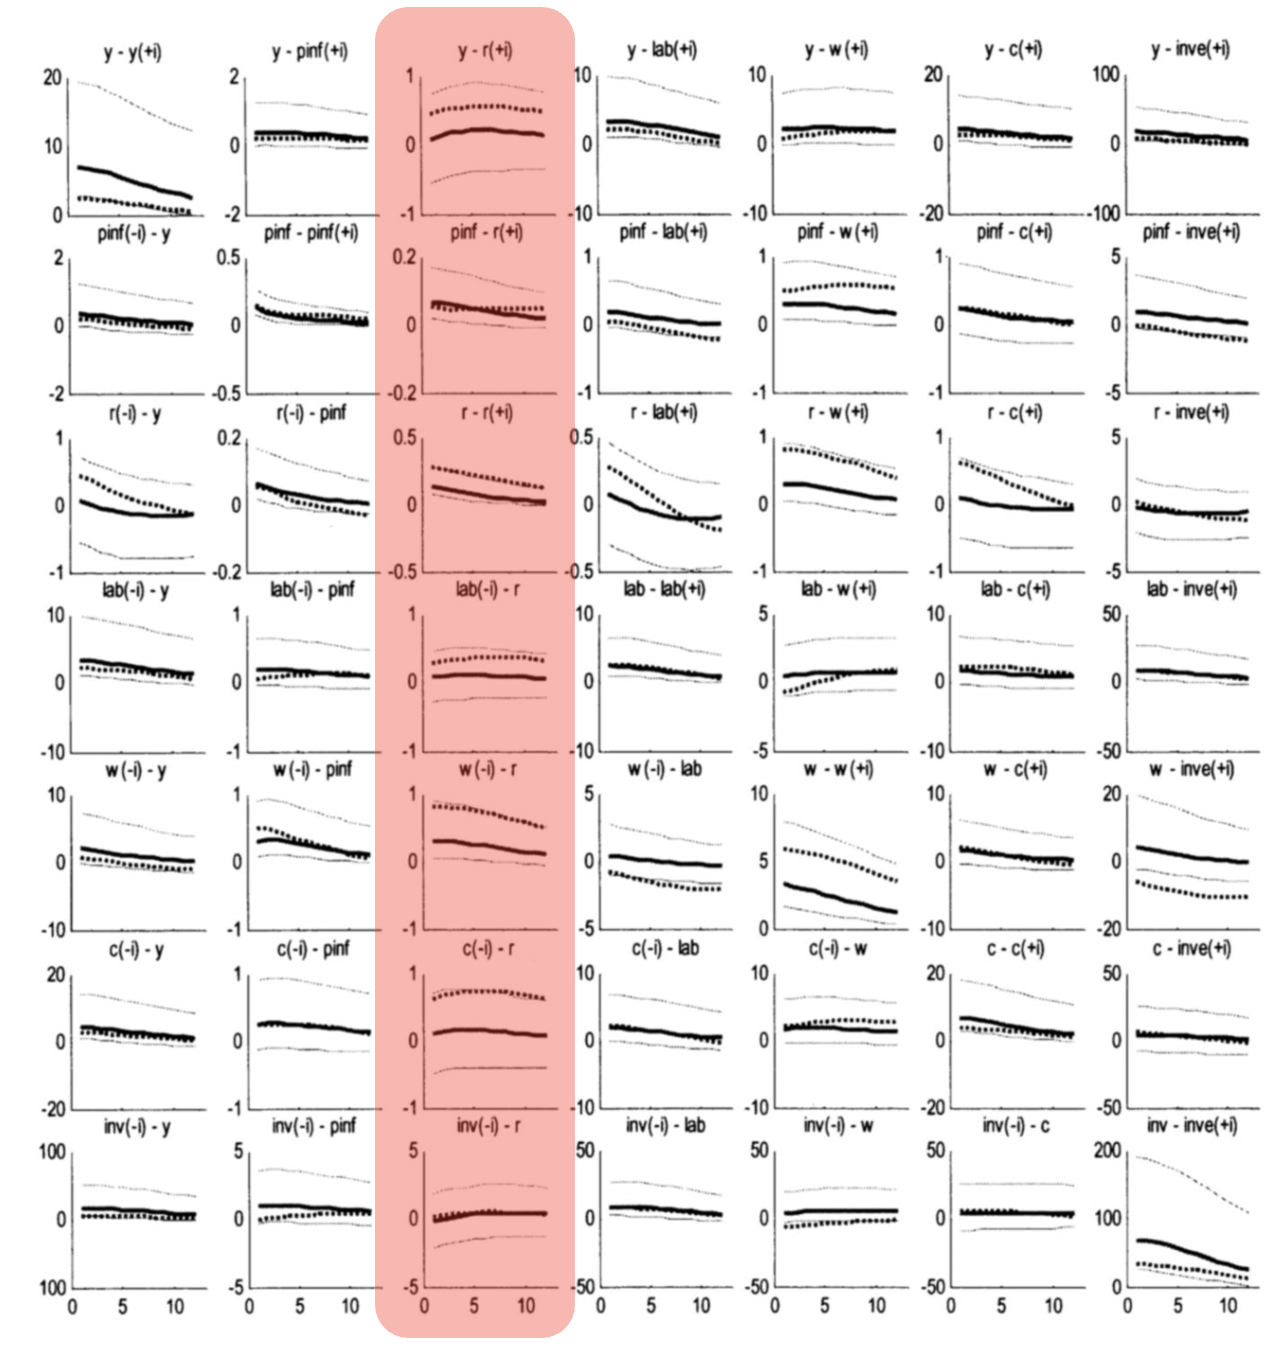
\includegraphics[width=0.55\linewidth]{images/cross_var.png}  
    \vspace{-0.4cm}  
    \caption{\small Comparison of Cross-Covariances: DSGE model VS data}  
    \label{fig:enter-label}  
\end{figure}  

\end{frame}   

\begin{frame}{Dimensionality Reduction Problem}
\begin{simplebox}{Limitation n°2 : On identification issues}
\textbf{(Too) High dimensional parameter space :} There are more shocks considered than endogenous variables ! (\texbtf{7} endogenous variable for \textbf{11} shocks)
\\ \textbf{Authors' Solution :} 
\begin{enumerate}
    \item Categorization : shocks are split between temporary and persistent shocks
    \item Independence:  All shocks are assumed to be uncorrelated
\end{enumerate}
\end{simplebox}
\end{frame}

\begin{frame}
	\centering
	
\includegraphics[width=1.4\linewidth]{images/thank-you.jpg}
\end{frame}

\appendix 

\begin{frame}{References}
  \printbibliography  
\end{frame}  


\end{document}